\documentclass[a4paper]{article}

\usepackage[utf8]{inputenc}
\usepackage[portuges]{babel}
\usepackage{indentfirst}
\usepackage{graphicx}
\usepackage{float}
\usepackage{caption}
\usepackage{subcaption}
\usepackage[T1]{fontenc}
\usepackage{listings}
\usepackage{amsmath}
\usepackage{mathtools}
\renewcommand{\familydefault}{\sfdefault}


\title{Projeto de Computação Gráfica - Fase 3}
\author{Diogo Braga A82547 \and João Silva A82005 \and Ricardo Caçador A81064
\and Ricardo Veloso A81919}
\date{\today}

\begin{document}

\maketitle

\begin{abstract}
Neste relatório é apresentada a terceira fase dum projeto no qual a intenção é desenvolver um mecanismo baseado em gráficos 3D e fornecer exemplos de uso que mostrem o seu potencial. Este projeto é desenvolvido no âmbito da unidade curricular de Computação Gráfica.
\end{abstract}


\newpage

\tableofcontents


\newpage

\section{Introdução}
\label{sec:intro}



\section{Estrutura da Pasta do Projeto}
\label{sec:estrutura}


\newpage

\section{Parser XML}
\label{sec:parser}

\subsection{Ficheiro}
\label{sec:ficheiro}

Devido aos requerimentos desta fase foi necessário alterar o ficheiro XML que provinha da segunda fase. As alterações aconteceram devido, por exemplo, à necessidade de incluir no ficheiro os pontos de controlo que, mais tarde gerado, dariam como resultado a curva de Catmull-Rom.

Importante referir que também nesta fase todos os sub-grupos herdam as transformações geométricas presentes no grupo ao qual pertencem. Nesta fase, estas transformações são: translações, rotações e escalas.

As escalas mantêm o mesmo funcionamento da fase anterior. Por outro lado, as translações e as rotações têm funcionamentos diferentes.

As translações funcionam tendo em conta um conjunto de 8 pontos que define uma curva de Catmull-Rom, e uma compontente \textit{time} que define o tempo que o objeto demora a realizar a curva. No caso das rotações, estas podem estabelecer o ângulo através da componente habitual \textit{angle}, ou através da componente \textit{time}.

Na figura \ref{img:ficheiro_parser} é possível visualizar um excerto do ficheiro XML referente à Terra e à Lua.

\begin{figure}[H]
\centering
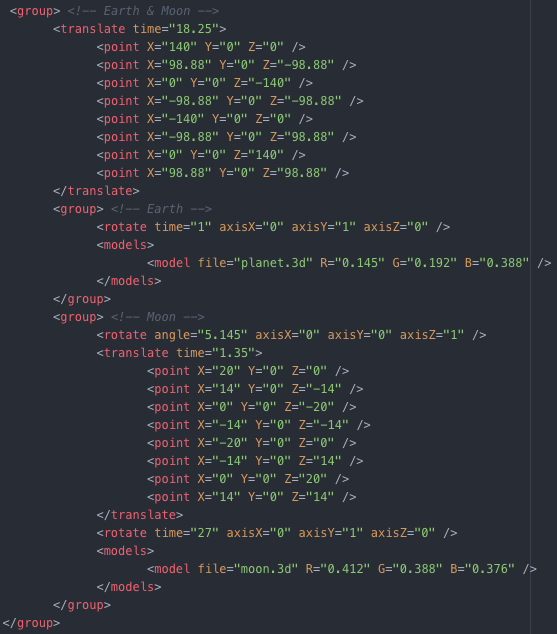
\includegraphics[scale=0.50]{ficheiro_parser.png}
\caption{Exemplo dum ficheiro usado no Parser.}
\label{img:ficheiro_parser}
\end{figure}

\subsection{Funcionamento}
\label{sec:funcionamento}



\section{Estruturas de Dados}
\label{sec:estruturasdados}



\section{Generator}
\label{sec:generator}

\subsection{Bezier Patches}
\label{sec:bezier}



\section{Engine}
\label{sec:engine}

\subsection{Catmull-Rom Cubic Curves}
\label{sec:catmullrom}


\subsection{VBOs}
\label{sec:vbos}



\section{Scenes}
\label{sec:scenes}


\section{Conclusão}
\label{sec:conclusao}


\section{Bibliografia}
\label{sec:bibliografia}


\end{document}
